\documentclass{article}
\usepackage[margin=1in]{geometry}
\usepackage{amsmath, amssymb, amsthm}
\usepackage[margin=1in]{geometry}
\usepackage{authblk}
\usepackage{hyperref}
\usepackage{xcolor}
\usepackage{graphicx}
\usepackage{enumitem}
\usepackage{bbm}
\usepackage{listings}
\usepackage{cleveref}
\usepackage{subcaption}

\DeclareMathOperator*{\R}{\mathbb{R}}
\DeclareMathOperator*{\E}{\mathbb{E}}
\DeclareMathOperator*{\Pz}{\mathcal{P}_{z^*}}
\DeclareMathOperator*{\Mpq}{\max \{p, q\}}

\definecolor{teal}{rgb}{0.0,.5,.5}
\newcommand{\teal}[1]{{\color{teal}{[{\bf teal:} #1]}}}

\newtheorem{theorem}{Theorem}
\newtheorem{lemma}[theorem]{Lemma}

\crefname{section}{Section}{Sections}
\crefname{equation}{Equation}{Equations}
\crefname{theorem}{Theorem}{Theorems}
\crefname{lemma}{Lemma}{Lemmas}
\crefname{listing}{Listing}{Listings}
\crefname{figure}{Figure}{Figures}

\graphicspath{{graphics/}}

\renewcommand{\lstlistingname}{Algorithm}% Listing -> Algorithm
\lstset{%
    basicstyle=\small\ttfamily,
    escapechar=~,
    frame=single,
    keywordstyle=\bfseries,
    keywords={input,output,foreach,return,if,in,then,do},
    mathescape=true,
    morecomment=[l][\color{blue}]{\#},
    numbers=left,
    xleftmargin=.04\textwidth
}

\title{Filter Bubbles}
\author{Indu Ramesh and R. Teal Witter}
\date{\today}

\begin{document}

\maketitle

%\section*{Proposal}

\subsection*{Motivation and Previous Work}

On the surface, the prominence of social media seems like it could make 
the world more connected, and expose users to a dizzying variety of diverse
ideas. However, recent studies have suggested social media encourages the
opposite, separating individuals into groups unable to find agreement, thereby
polarizing society. A popular explanation for this phenomenon has been coined 
the filter bubble-- the idea that the content displayed on 
users’ feeds is social
media networks is simply an echo chamber that prevents people from accessing a
diverse array of viewpoints. Since user feed content is constrained by metrics
that aim to increase user engagement and ad revenue (i.e. friends’ and 
followers’
views, internet search history, user location, etc.), social media companies
explicitly incentivize users to pay preferential attention to like-minded
content. In this manner, users end up living in a ‘filter bubble’ of their own
ideas. Filter bubbles have been blamed for the spread of misinformation in
Brexit, the 2016 U.S. presidential election, and increased 
distrust in democracy.

Chitra and Musco’s paper aimed to provide a rigorous mathematical theory
solidifying filter bubbles’ emergence, studying user opinion dynamics within
social networks \cite{chitra_analyzing_2020}.
Each network is modeled as a weighted graph per a \emph{stochastic
block model}. Each node corresponds to an individual, and edges between nodes
correspond to social relationships. The “stochastic” aspect is as follows: the 
probability of two nodes being connected is higher 
when the nodes are in the same
community, and lower in different communities. Relationships between users with
increased interactions (i.e. their respective stories pop up in their news feeds
more often) have higher edge weights; relationships where users barely interact
are assigned low edge weights. Chitra and Musco 
adapted the \emph{Friedkin-Johnsen model}
to address opinion dynamics,  augmenting each 
node with an opinion, a real number
in the interval [-1,1]. As time passes, each node’s opinion value is updated
based on the average opinion of their neighbors and connections in the social
network. Polarization is represented by the variance of opinions within the
network, where opinions are represented as a $n$-dimensional vector.

To formalize social media companies’ roles in creating filter bubbles,
Chitra and Musco studied the influence of an important outside actor on 
the Friedkin-Johnsen model: the \emph{network administrator}. The network
administrator’s job is to minimize disagreement among users by 
modifying the edge weights of the graph such that users interact
with more content from users with similar opinions. The network
administrator’s modifications are subject to certain constraints;
for instance, they cannot change the degree of any vertex, 
and they can only modify edge weights by a small amount. 
Chitra and Musco ran experiments on the social networks Twitter
and Reddit to simulate the effect of a network administrator
on polarization.

Their experimental results confirm filter bubble theory. 
That is, a social network modeled by the stochastic block 
model is, with high probability, already in a state of \emph{fragile consensus}. 
Though a network may exhibit low polarization, a minor change in 
edge weights can cause a shift to high polarization. 
For example, when the network administrator changed only 
$40\%$ of the total edge weight in the graph, polarization 
increased by a $40$-fold factor. Chitra and Musco also demonstrated 
a simple fix to this phenomenon. Recall that the network 
administrator’s object was to minimize disagreement:
$\min_G D_z$.
They proposed a solution to add a regularization term to the objective
(ridge regression): 
$\min_G D_z + \lambda w^Tw$
Their solution constrained the increase in polarization by a network
administrator to $4\%$. 

\subsection*{Research Questions}

We propose the following further research directions to
extend Chitra and Musco’s work. 

\begin{enumerate}
    \item \emph{Formalizing the network administrator’s role}: Chitra and Musco informally assert that the network 
    administrator’s role is to minimize disagreement. Can we prove, formally, that this is the case-- i.e. 
    solve the optimization problem? Could we prove that a “simpler” or “natural” action by the network administrator-- i.e. maintaining the overall weight of the graph, but increasing the weights between highly agreeable neighbors and decreasing the weights between disagreeing neighbors-- still converges 
    to a more highly polarized vector of opinions? Can we prove this in a stochastic block model? What 
    about other models? 
    \item \emph{Dealing with outside attacks}:
    Could we model some sort of 
    attack by an outside actor on increasing polarization? 
    An example is Cambridge Analytica’s role in the 2016 
    presidential election to sway undecided voters toward 
    electing Trump, popularized by the Netflix documentary 
    “The Great Hack.” Here’s a simple idea: at each time step, 
    introduce a new ‘fake’ node with an opinion. How many fake nodes,
    and how strong of opinions, would we have to introduce to 
    converge to a final set of opinions with higher polarization,
    and how many time steps would that take?
    \item \emph{Investigating Bimodality}:
    Some suggest that polarization, 
    defined by Chitra and Musco as the variance of the n opinions 
    of the network’s users, might not actually be what’s increasing
    as much as Chitra and Musco experimentally demonstrate. 
    What’s actually going on may be more accurately explained by increasing \emph{bimodality}, where opinions converge in clusters around two centers, as opposed to opinions being further away from where we started.  In other words, we can modify Chitra and Musco’s question to: “How sensitive are social networks to bimodality?” 
    We propose formally defining bimodality and seeing 
    if we can obtain a similar result to the “fragile consensus”
    linear algebraic results by Chitra and Musco. 
\end{enumerate}

%\section*{Network Administrator Actions}

\begin{minipage}{\linewidth}
\begin{lstlisting}[caption={Opinion formation with network administrator.}, label={lst:update}]
    input: adjacency matrix $A_0$ of dimension $n\times n$,
           initial set of opinions $s$ with $s_i \in (-1,1)$ for $i \in [n]$,
           number of iterations $T$ to run
    output: a set of equalibrium opinions $z^{(T)}$
    $z^{(0)} \gets s$
    foreach $t$ in $\{0,\ldots, T\}$ do
        $D \gets$ degree matrix of $A_t$
        $z^{(t)} \gets (D+I)^{-1} (A_t z^{t-1} + s)$
        $A_t \gets$ network administrator modifications of $A_{t-1}$
    return $z^{(T)}$
\end{lstlisting}
\end{minipage}

``Natural'' network administrator actions:
\begin{enumerate}
    \item For each node $u \in [n]$,
    add $\epsilon > 0$ to the weight of the adjacent edge closest
    in current opinion to $u$
    and subtract $\epsilon$ from the weights of the adjacent
    edges furthest in current opinion from $u$ subject to the
    constraint that each edge has at most $\delta > 0$ weight.
\end{enumerate}

\subsection*{To Do}
\begin{itemize}
    \item[\checkmark] Code up \autoref{lst:update}.
    \item[\checkmark] Implement a slightly easier version of the first network
    administrator action.
    \item Implement the full version of the first network
    administrator action.
    \item Understand Equation 14 in \cite{chitra_analyzing_2020}.
    \item Find about an administrator modification that
    can be written in matrix notation.
\end{itemize}
% chktex-file 46

\section{Introduction}

Over the past decade, social media has transformed societal interaction. In theory, social media allows individuals and groups access to a diverse array of ideas. However, recent studies suggest that social networks are associated with societal polarization, separating individuals into groups unable to find agreement \cite{greatergood}. 

A popular explanation for this phenomenon is the emergence of \emph{filter bubbles}, a term coined by internet activist Eli Pariser \cite{Pariser}. Filter bubbles reflect the idea that users’ news feeds in social media networks are simply echo chambers that prevent individuals from accessing a variety of viewpoints. Since user feed content is constrained by metrics that aim to increase user engagement and ad revenue (i.e. friends’ and followers’ views, internet search history, user location, etc.), social media companies explicitly incentivize users to pay preferential attention to like-minded content. In this manner, users end up living in a ‘filter bubble’ of their own ideas. Filter bubbles have been blamed for the spread of misinformation in Brexit, the 2016 U.S. presidential election, and increased distrust in democracy \cite{filterbubble}.

In this project, we study \emph{polarization} in social networks, aiming to advance a mathematical theory behind the formation of filter bubbles. 

\subsection{Related Work}

Through studying various metrics and models of polarization, a mathematical theory has begun to emerge. We give a summary of interesting recent approaches and results. 

In \cite{Dandekarpnas}, Dandekar et al. studied the idea of \emph{biased assimilation}: when given mixed evidence on a complex issue, individuals use that evidence to support their innate opinion, arriving at a more extreme version of their original opinion. They provided evidence that in simple models of social networks, DeGroot's model of opinion formation \cite{Degroot} results in convergence at a less diverse set of opinions, falling short of explaining polarization. They also analyzed the effects of three internet content recommendation algorithms on polarization, showing that if individuals start out sufficiently biased, these algorithms lead to increased polarization.

In \cite{chitra20analyzing}, Chitra and Musco studied social media companies’ roles in creating filter bubbles using a related model of opinion formation, the Friedkin-Johnsen model \cite{fj}. They explored the effect of adding an important outside actor to the picture: the \emph{network administrator}. The network administrator’s job is to minimize disagreement among users by modifying the edge weights of the graph such that users interact with more content from users with similar opinions. In their model, the network administrator’s modifications are subject to certain constraints: the administrator cannot change the degree of any vertex, and can only modify edge weights by a small amount. Chitra and Musco ran experiments on the social networks Twitter and Reddit to simulate the effect of a network administrator on polarization. Their experimental results confirm filter bubble theory, and they show that there is a network administrator action that leads to increased polarization.

Other formulations and solutions to the polarization problem have been studied. In \cite{muscomusco}, Musco et al. asked: what is the \emph{topological structure} of a network that minimizes both polarization and disagreement, given an opinion dynamics model? They posed this question as an optimization problem, and gave a polynomial-time algorithm that approximates the optimum for a fixed graph. In \cite{algorithmfilterbubbles}, Matakos et al. formulated polarization as an influence maximization problem, providing an approximation algorithm to break up filter bubbles. 

Finally, consider that the work we mentioned has addressed the question: how sensitive are networks to polarization? Chitra and Musco's results in \cite{chitra20analyzing} suggest that many networks are in a state of \emph{fragile consensus}. The Netflix documentary ``The Great Hack" \cite{Netflix} discusses Cambridge Analytica’s role in the 2016 presidential election, swaying undecided voters toward electing Trump through targeted intervention on Facebook. Could we exploit this sensitivity, and model some sort of attack by an outside actor on increasing polarization? 


\subsection{Overview of Results}

In this project, we study polarization in the Friedkin-Johnson (FJ) dynamics model, formally defined below.
In \cref{sec:experiments}, we present empirical results
on the impacts of several additions to the FJ opinion formation
process.
Notably, we introduce two natural network administrator
actions and describe their effects on social networks.
In \cref{sec:theory}, we extend the results of
\cite{chitra20analyzing}.
In particular, we show that the polarization of the
equilibrium opinions after running FJ dynamics
on the Stochastic Block Model (SBM) defined below
converges with high probability for any mean-centered
innate opinions (rather than the half 1, half -1 innate
opinions considered before).
When the graph is in the special case of 
an Erdős–Rényi our bounds are even stronger.
Finally, we discuss our work and provide directions
for future work in \cref{sec:conclusion}.




% chktex-file 46

\section{Background and Preliminaries}
The formulation of the polarization problem we study focuses specifically on mathematical models of opinion formation in social networks. 

Social networks arise randomly, with individuals developing connections based on social groups. Thus, the natural mathematical representation of a social network is a graph. Each node represents an individual and an edge represents a friendship or connection in the network. Edges have weights associated with the extent of their friends' influence on their opinions-- in other words, the ``closeness" of the friendship. In a real-life social network like Facebook, a higher edge weight between users corresponds to a increased interactions between those users (e.g. their respective stories pop up in their news feeds more often). 

\subsection{The Stochastic Block Model}

In this project, we use a random graph model termed the Stochastic Block Mode (SBM) to construct a graph representing a social network. The SBM is a common generative model seen in numerous fields, including statistics, theoretical computer science, and machine learning \cite{sbm}. We refer the interested reader to \cite{sbm} for a comprehensive survey of applications of the SBM. 

An SBM graph $G$ has $n$ vertices, divided into several communities.
The probability that there is an edge between two nodes in the same community
is $p$ while the probability there is an edge between two nodes
in different communities is $q$.

Often, we have that $p \geq q$, to model the idea that relationships
within communities are more likely than relationships between
communities.
However, there are some real-world situations where $p \leq q$.
Consider a patient-doctor network and the way opinions of
e.g. a vaccine are formed.
Connections representing conversations about a vaccine
are most likely between a doctor and a patient and less
likely between patient and patient or doctor and doctor.
Such a model is particularly relevant to
the acceptance of COVID-19 vaccines \cite{hoff2020patient-doctor}. When $p=q$, the SBM is known as an Erdős-Rényi graph.

\subsection{Opinion Formation}
There are two main models of opinion formation in social
networks.
The input to both models is a social network
given by a graph and an innate (starting) opinion for each
node in the graph.
That is, each node $i$ has an innate opinion
$s_i$ and expressed opinion (that changes according
to the respective model) $z_i$
where $s_i, z_i \in [-1, 1]$.

\paragraph{DeGroot's Model:} Perhaps the most popular model of opinion dynamics studied, DeGroot's model updates a node's opinion with the weighted average of its expressed opinion and its friends opinions. Formally,
\begin{align}
    z_i^{(t)} = \frac{z_i^{(t-1)} + \sum_{j \neq i} w_{ij}z_j^{(t-1)}}{d_i + 1}
    \nonumber
\end{align}

where $z_i^{(t)}$ is the opinion of node $i$ at iteration $t$,
$z_i^{(t-1)}$ is the opinion of node $i$ in the previous iteration,
and $d_i$ is the degree of node $i$ in the graph.
\medskip \medskip

\paragraph{Friedkin-Johnsen Model:} The Friedkin-Johnsen (FJ) opinion dynamics model is similar to DeGroot's Model but, instead
of averaging with the node's own expressed opinion, averages
with the innate opinion.
Intuitively, FJ opinions are more `stubborn.'
Formally,

\begin{align}\label{eq:updateruleFJ}
    z_i^{(t)} = \frac{s_i + \sum_{j \neq i}
    w_{ij}z_j^{(t-1)}}{d_i + 1}
\end{align}

where $z_i^{(t)}$ is the opinion at iteration $t$, $s_i$ is the innate opinion of node $i$, and $d_i$ is the degree of node $i$ in the graph.

We will use FJ dynamics because
\cite{Dandekarpnas} have shown that polarization
(formally defined in the next section)
always converges in DeGroot's model.

\subsection{Measuring Polarization}

One measure of polarization with a natural mathematical interpretation is is the \emph{network disagreement} index. In \cite{Dandekarpnas}, a process is viewed as \emph{polarizing} if it increases the network disagreement index. In a social network graph $G = {V,E,w}$, the network disagreement index is calculated as follows:

\begin{align}
    \eta(G,x) = \sum_{i,j \in E} w_{ij}(x_i - x_j)^2 
    \nonumber
\end{align}

where $x_i$ and $x_j$ are the opinions at nodes $i$ and $j$.

In \cite{chitra20analyzing}, Chitra and Musco add some structure to the measure of polarization. They define polarization as the \emph{variance} of a set of opinions. For a vector of $n$ opinions ${z} \in [-1,1]$, let

\begin{align}
    \E[{z}] = \frac{1}{n}\sum_{j=1}^n x_j 
    \nonumber
\end{align}

where $z_j$ is the mean opinion of {z}. Then, polarization, $P_z$ can be defined as:

\begin{align}
    P_z = \sum_{i=1}^n (x_i - \E[{z}])^2
    \nonumber
\end{align}

Another measure is \emph{bimodality}.
Instead of simply of measuring the difference from the mean,
bimodality gives a sense for whether opinions are centered
at two different means.
Formally, the bimodality coefficient is given by

\begin{align}
    \beta = \frac{\gamma^2 + 1}{\kappa}
    \nonumber
\end{align}

\noindent where $\gamma$ is the \emph{skewness} (third standardized moment) and $\kappa$ is the \emph{kurtosis} (fourth standardized moment). 
Measuring bimodality is particularly relevant to
the modern political situation in the United States
\cite{bromley2017tale}.

\subsection{Linear Algebraic Interpretation of FJ Opinion Dynamics} 
To analyze polarization on an SBM graph, it is helpful to have a linear algebraic interpretation of FJ opinion dynamics. We follow the approach in  \cite{chitra20analyzing}.

Let $A \in R^{n \times n}$ be the adjacency matrix of $G$, where $A_{ij} = A_{ji}$ since the graph is undirected. Let $D$ be a diagonal matrix where $D_{ii} = d_i$. That is, each diagonal entry is equal to the degree of node $i$, and the other entries are 0's. Finally, let $L = D - A$ be the \emph{Laplacian} of $G$. Recall that ${s}$ is the innate opinion vector of all nodes in $G$.
It is not too hard to see that \cref{eq:updateruleFJ} is equivalent to

\begin{align}\label{updaterulelinalg}
    {z}^{(t)} = (D + I)^{-1}(A{z}^{(t-1)} + {s})
\end{align}

where $ {z}^{(t)} = \begin{bmatrix} z_1^{(t)} & z_2^{(t)} & \cdots & z_n^{(t)} \end{bmatrix}$. 

Let ${z}^{(*)}$ be the final equilibrum opinion vector after $t$ time steps. Then 

\begin{align}\label{zstar}
    {z}^{(*)} = (L + I)^{-1}{s}.
\end{align}


% chktex-file 46

\section{Experiments}\label{sec:experiments}

It is often challenging to mathematically analyze
variations on the opinion formation process, so we simulate
them instead.
The variations we consider include:
network administrator actions, attack nodes,
imbalanced innate opinions, and three (rather than two)
blocks in the Stochastic Block Model (SBM).

\cref{lst:overview} presents the baseline
pseudocode we use for our experiments.

\begin{minipage}{\linewidth}
\begin{lstlisting}[caption={Opinion formation.}, label={lst:overview}]
input: adjacency matrix $A_0$ of dimension $n\times n$,
        innate set of opinions $s$ with $s_i \in [-1,1]$ for $i \in [n]$,
        number of iterations $T$ to run
output: a set of equalibrium opinions $z^{(T)}$
$z^{(0)} \gets s$
foreach $t$ in $\{0,\ldots, T\}$ do
    $D \gets$ degree matrix of $A_t$
    $z^{(t)} \gets (D+I)^{-1} (A_t z^{t-1} + s)$
    $A_t \gets$ network administrator modifications of $A_{t-1}$
return $z^{(T)}$
\end{lstlisting}
\end{minipage}

\subsection{Extreme Administrator Action}
The first administrator update we consider is
a simple, intuitive update rule: add weight to the neighbor
with closest opinion and subtract the same weight
from the neighbor with furthest opinion.

\cref{lst:extreme} presents the pseudocode for the update.
The overall weight of friendships is preserved in the
graph, but many friendships disappear and some nodes even
lose their connections altogether.

\begin{minipage}{\linewidth}
\begin{lstlisting}[caption={Extreme Administrator Update.}, label={lst:extreme}]
input: adjacency matrix $A$ of dimension $n\times n$,
        expressed opinions $z^{(t)}$,
        maximum edge change $\epsilon$ per iteration
output: modified adjacency matrix $A'$
$A' \gets$ all-zero $n \times n$ matrix
foreach $u$ in $[n]$ with more than one neighbor do
    c $\gets$ neighbor with closest opinion to $u$
    f $\gets$ neighbor with furthest opinion to $u$
    $\Delta \gets \min \{ \epsilon, A_{u,f}\}$
    $A'_{u,f} \gets A'_{f,u} \gets A_{f,u} - \Delta$
    $A'_{u,c} \gets A'_{c,u} \gets A_{c,u} + \Delta$
return $A'$
\end{lstlisting}
\end{minipage}

\cref{fig:extreme} shows the ratio of remaining
friendships, bimodality, and polarization in four
different pairs of social networks and innate opinions.
The SBM social network in both \cref{fig:extreme}
and \cref{fig:scale} is the same random network
on $n=100$ in order to preserve consistency.
We use $p=30/n$ and $q=5/n$.

The ratio of remaining friendships with the extreme
update (green) drops quickly
across all four figures until it stabilizes around .1.
When the innate opinion is extremely polarized
(half 1, half -1) in \cref{fig:extremeextreme}
the final ratio of remaining friendships is even smaller.

Bimodality is highest with the extremely polarized
innate opinions (orange).
Otherwise, it stabilizes in the middle of the range.
Interestingly, the SBM
with two normal innate opinions centered
at .5 and -.5, respectively looks similar
to the Reddit and Twitter social networks.
This suggests that the bimodal SBM
is a good model for real-world social networks.
Polarization only
increases to 1 when innate opinions are extremely
polarized.
Otherwise, it slowly increases over time and stabilizes
near 0.

\begin{figure}[h]
    \centering
    \begin{subfigure}[b]{0.4\textwidth}
        \centering
        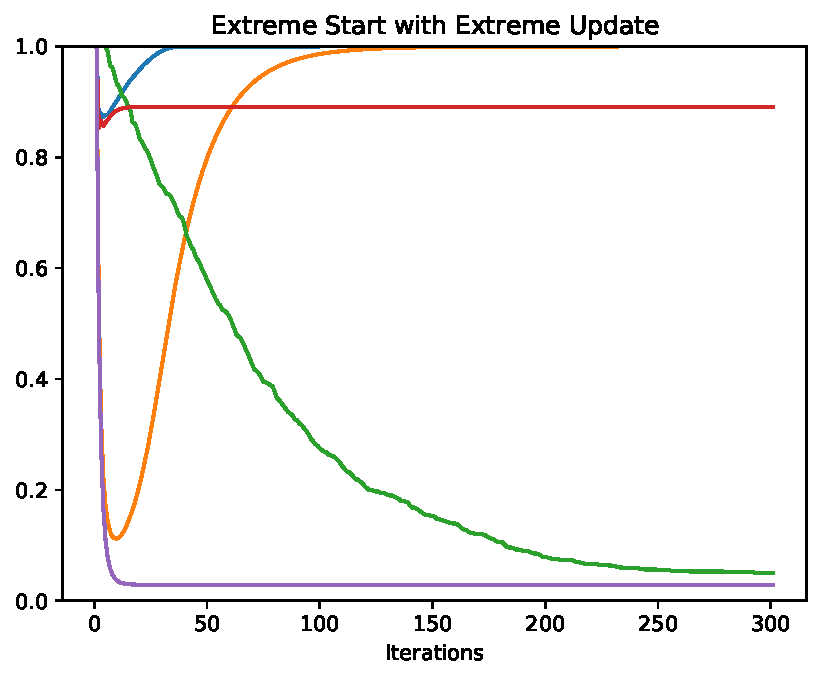
\includegraphics[width=\textwidth]{extremeextreme.pdf}
        \caption{SBM with half 1, -1 innate opinions.}
        \label{fig:extremeextreme}
    \end{subfigure}
    \begin{subfigure}[b]{0.4\textwidth}  
        \centering 
        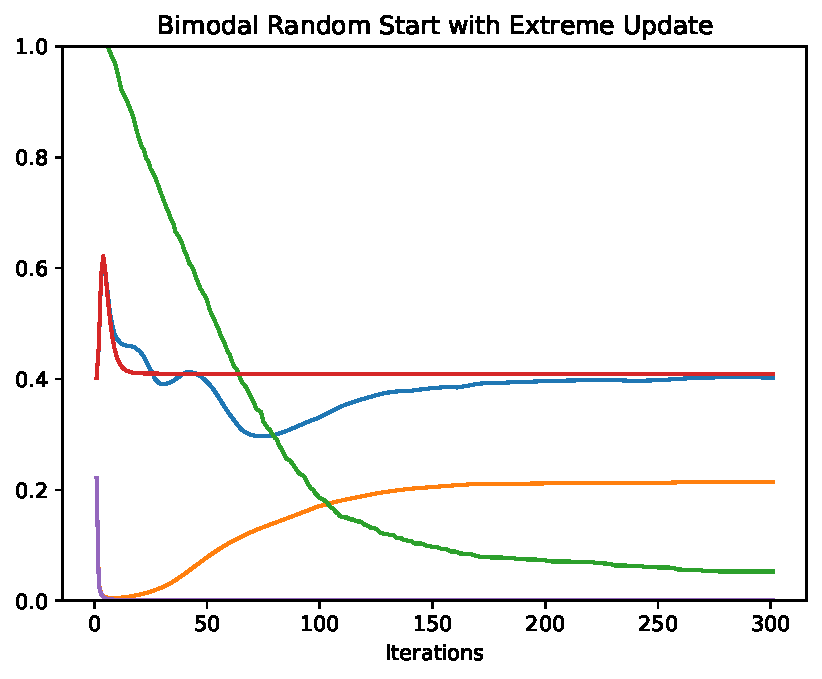
\includegraphics[width=\textwidth]{extremerandom.pdf}
        \caption{SBM with two scaled normal opinions.}
        \label{fig:extremerandom}
    \end{subfigure}
    \vskip\baselineskip
    \begin{subfigure}[b]{0.4\textwidth}   
        \centering 
        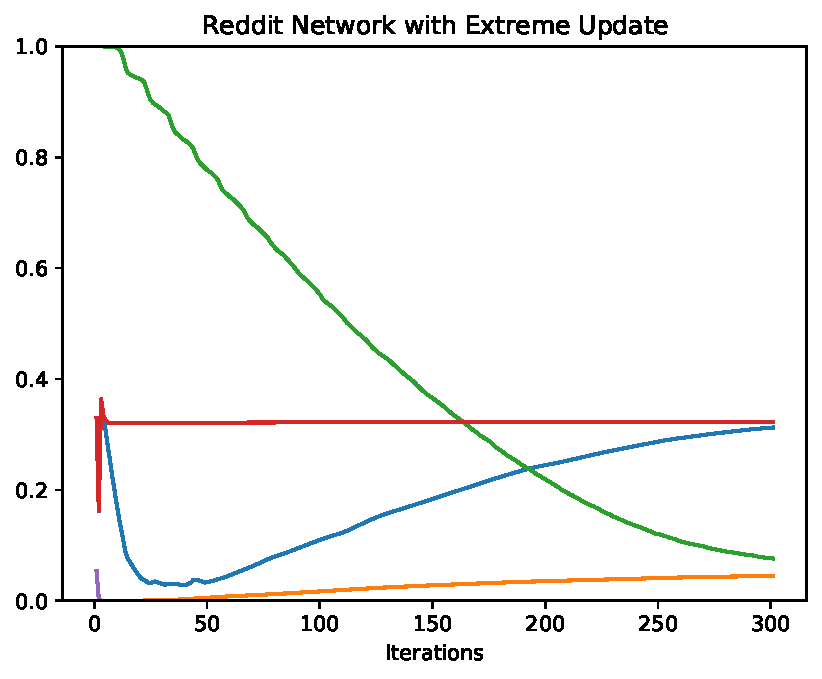
\includegraphics[width=\textwidth]{extremereddit.pdf}
        \caption{Posts on r/politics and other subreddits.}
        \label{fig:extremereddit}
    \end{subfigure}
    \begin{subfigure}[b]{0.4\textwidth}   
        \centering 
        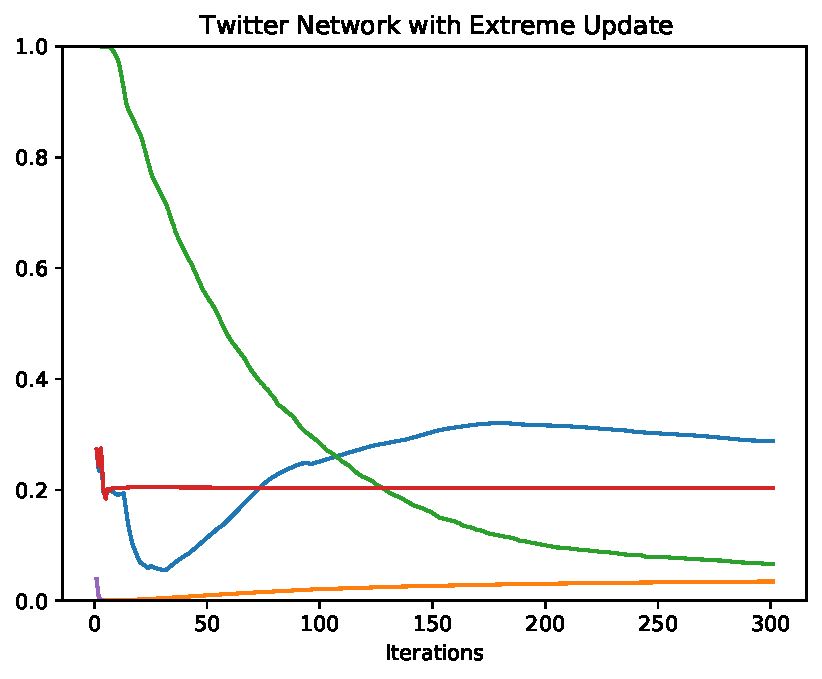
\includegraphics[width=\textwidth]{extremetwitter.pdf}
        \caption{2013 Delhi election opinions on Twitter.}
        \label{fig:extremetwitter}
    \end{subfigure}
    \caption{Difference between baseline and extreme administrator
    update on four different social network and opinion pairs.
    Brown corresponds to the ratio of remaining friendships in the baseline
    opinion formation process, green to friendships in the extreme update,
    red to bimodality in baseline, blue to bimodality in extreme,
    purple to polarization in baseline, and orange to polarization in extreme.}
    \label{fig:extreme}
\end{figure}

The extreme administrator update is a naive approach
to the natural mechanism social media platforms use
to boost engagement: increase exposure to content
similar in nature to user preferences
and simultaneously decrease exposure to content
dissimilar to user preferences.

While the overall weight (interpreted as time
by \cite{chitra20analyzing}) stays constant,
the individual level weight can move from one
node to another.
This combined with the elimination of friendships
suggest that the extreme update is not a reasonable
administrator action.
Nonetheless, analyzing it provides insight into an
intuitive idea and the extremes of a potential
administrator action.

\subsection{Scaled Administrator Action}
The other administrator action we consider
is a less extreme variation.
Instead of subtracting weights from edges
and risking eliminating connections,
the scaled administrator only adds weights
and then normalizes to preserve the 
weights of each row.
The unfortunate result is that the
matrix is no longer symmetric.

\cref{lst:scaled} presents the pseudocode for
the scaled update.
The idea is that we want to add more weight
to edges close in opinion and less to edges far
in opinion.
We do this by taking 2 (the most extreme possible
difference between opinions) minus the absolute
difference in opinion for each node
and multiplying by $\epsilon$.
(Empirically, varying $0 \leq \epsilon \leq 1$
has a limited impact on the resulting figures.)
If two nodes have the same opinion, we add
$2\epsilon$; if their opinions are as far
apart as possible, we do not add any weight.

\begin{minipage}{\linewidth}
\begin{lstlisting}[caption={Scaled Administrator Update.}, label={lst:scaled}]
input: adjacency matrix $A$ of dimension $n\times n$,
        expressed opinions $z^{(t)}$,
        maximum edge change $\epsilon$ per iteration
output: modified adjacency matrix $A'$
$A' \gets$ copy of $A$
foreach $u$ in $[n]$ with more than one neighbor do
    $\Delta \gets \epsilon (A_{u,:} > 0)\times (2 - |z^{(t)}-z^{(t)}_u|)$ # resulting $\color{blue}n \times 1$ vector
    norm $\gets |\textrm{neighbors}|/(\sum_{v \in [n]}A_{u,v}+\Delta_v)$
    $A'_{u,:} \gets (A_{u,:}+\Delta)/$norm
return $A'$
\end{lstlisting}
\end{minipage}

\cref{fig:scale} shows bimodality and 
polarization as a function of iterations
for the baseline and scaled administrator update.
Notably, the time until the trends converge
is substantially smaller than the times
for the extreme update.

Across all four figures,
polarization reaches 0 fairly quickly.
The difference between the baseline and scaled update
is that the scaled bimodality is higher
most clearly in \cref{fig:scaletwitter}
but also in \cref{fig:scaleextreme}
and \cref{fig:scalereddit}.
Curiously, the bimodal SBM shows
no discernible difference between the baseline
and the scaled update.

\begin{figure}[h]
    \centering
    \begin{subfigure}[b]{0.4\textwidth}
        \centering
        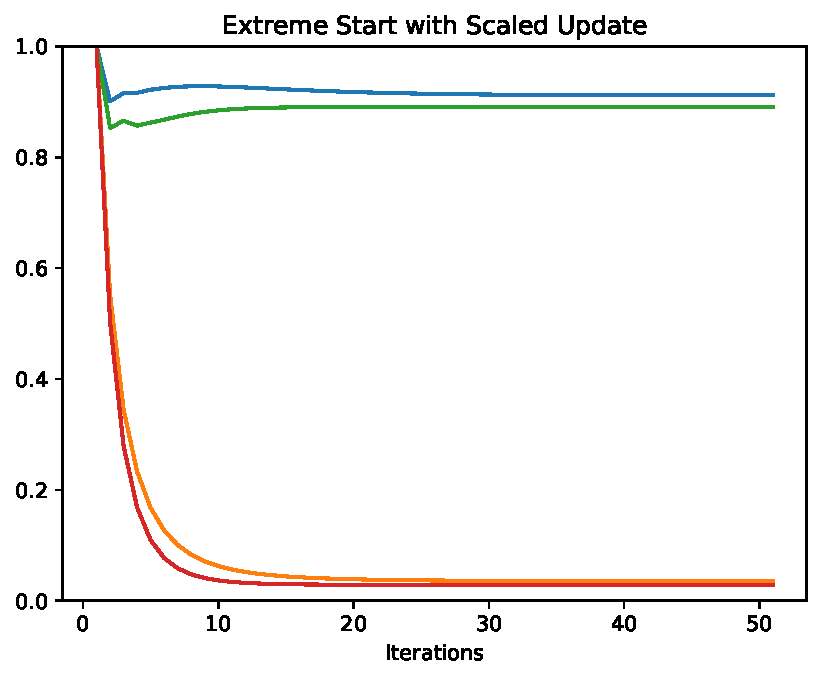
\includegraphics[width=\textwidth]{scaleextreme.pdf}
        \caption{SBM with half 1, -1 innate opinions.}
        \label{fig:scaleextreme}
    \end{subfigure}
    \begin{subfigure}[b]{0.4\textwidth}  
        \centering 
        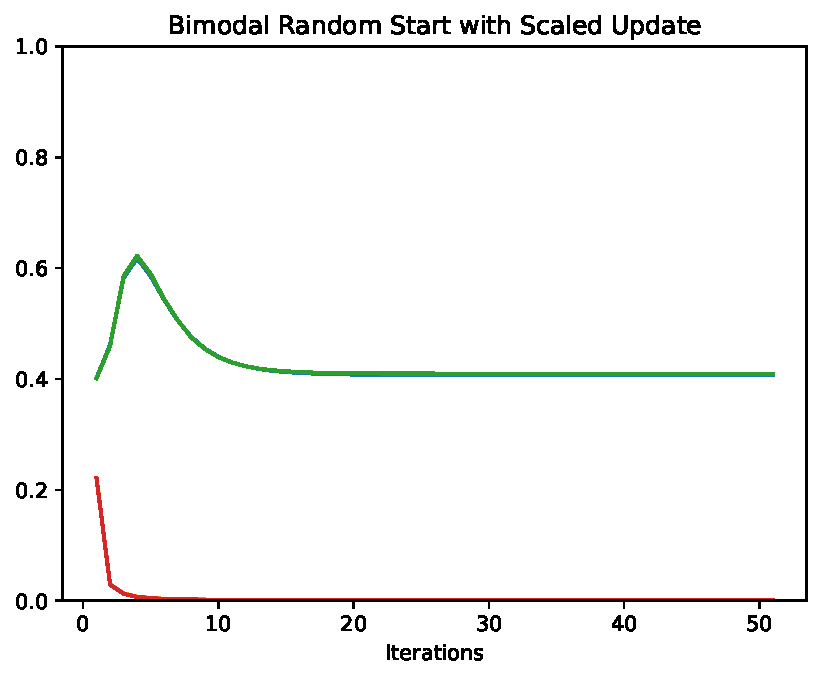
\includegraphics[width=\textwidth]{scalerandom.pdf}
        \caption{SBM with two normal opinions.}
        \label{fig:scalerandom}
    \end{subfigure}
    \vskip\baselineskip
    \begin{subfigure}[b]{0.4\textwidth}   
        \centering 
        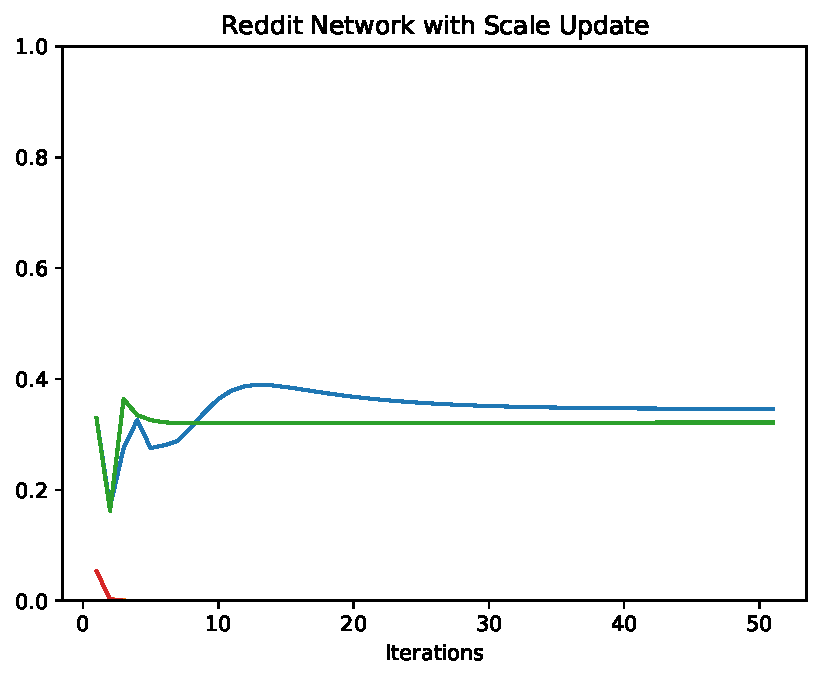
\includegraphics[width=\textwidth]{scalereddit.pdf}
        \caption{Posts on r/politics and other subreddits.}
        \label{fig:scalereddit}
    \end{subfigure}
    \begin{subfigure}[b]{0.4\textwidth}   
        \centering 
        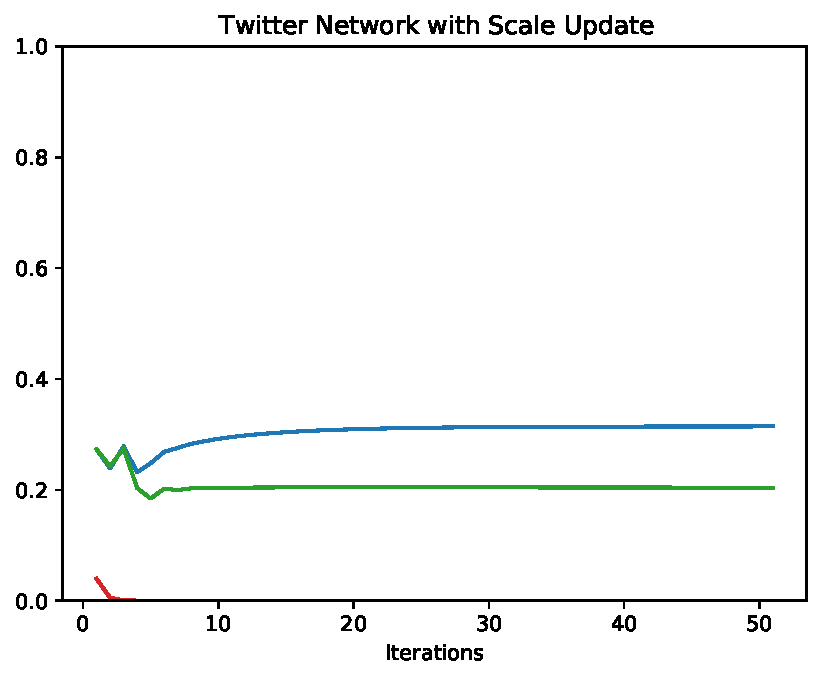
\includegraphics[width=\textwidth]{scaletwitter.pdf}
        \caption{2013 Delhi election opinions on Twitter.}
        \label{fig:scaletwitter}
    \end{subfigure}
    \caption{Difference between baseline and scaled administrator
    update on four different social network and opinion pairs.
    Green corresponds to bimodality in the baseline update,
    blue to bimodality in the scaled update,
    red to polarization in the baseline,
    and orange to polarization in the scaled update.}
    \label{fig:scale}
\end{figure}

The scaled update administrator action
takes a more subtle approach.
While the action boosts like-minded content,
the increase in bimodality is marginal
and the increase in polarization is negligible.

\subsection{Miscellaneous Variations}

In this section, we analyze the following variations:
attacker nodes with an extreme opinion that do not update
their own opinion, three stochastic blocks rather than two,
and an imbalanced opinion (1/3-2/3 vs 1/2-1/2).

\begin{figure}[h]
    \centering
    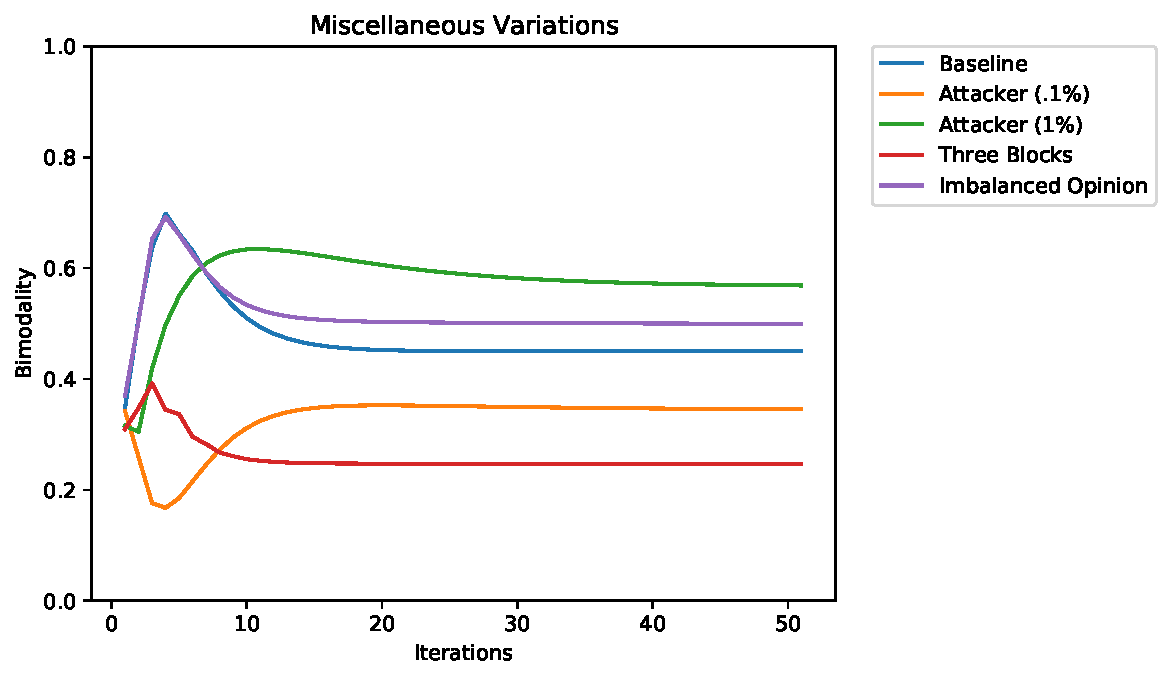
\includegraphics[width=.75\textwidth]{misc.pdf}
    \caption{SBM with half 1, -1 innate opinions.}
    \label{fig:misc}
\end{figure}

\autoref{fig:misc} shows the bimodality of each variation
on social networks with $n=1000$ nodes.
The imbalanced opinion is closest to the baseline,
maintaining essentially the same bimodality until the $10$th
iteration when the bimodality of the imbalanced opinion increases.
The attacker node that constitutes .1\% of the population
ironically seems to reduce bimodality.
The attacker nodes that constitute 1\% of the population
markedly increase bimodality as we would expect.
Finally, the three block model has the lowest bimodality.
This makes sense given that the three blocks are centered
at .5, 0, -.5 respectively rather than the more polarized
.5 and -.5.

%We experimentally evaluated two network administrator actions, updateExtreme and updateScale, on random graphs generated via the stochastic block model and two real-world networks. These real-world datasets have previously been utilized to study polarization in \cite{datasets}, \cite{muscomusco}, and \cite{chitra20analyzing}, and we obtained the datasets from those authors. 
%
%\subsection{Datasets}
%\paragraph{Twitter} is a graph with $548$ nodes and $3638$ edges. Nodes correspond to users who posted tweets about the Delhi legislative assembly elections of 2013, and edges represent user interactions debating that election. 
%
%\paragraph{Reddit} is a graph with $556$ nodes and $8969$ edges. Nodes represent users who posted in the r/politics subreddit. Edges correspond to users' posts in different subreddits. In particular, two users are connected by an edge if they have both posted in two subreddits (other than r/politics) during the given time period.
%
%\paragraph{}In both networks, each user has multiple opinions associated to them, analyzed via their posts. We used a similar data extraction method to \cite{chitra20analyzing}, averaging each opinion to give an equilibrium vector for each user. When all innate opinions are collected into vector $s$, the vector is mapped into the interval $[-1,1]$.
%
%\subsection{Network Administrator Actions}
%
%We describe the network administrator algorithms we implemented and experimentally evaluated. 
%
%\paragraph{updateExtreme} 
%\begin{enumerate}
    %\item For each node $u \in [n]$,
    %add $\epsilon > 0$ to the weight of the adjacent edge closest
    %in current opinion to $u$
    %and subtract $\epsilon$ from the weights of the adjacent
    %edges furthest in current opinion from $u$ subject to the
    %constraint that each edge has at most $\delta > 0$ weight.
%\end{enumerate}
%
%\paragraph{updateScale} 
%
%\subsection{Results}
% chktex-file 46
\pagebreak
\section{Theory}\label{sec:theory}
We present our theoretical results in this section.
We use the work of \cite{chitra20analyzing}
as a foundation for our results.

We consider the Stochastic Block Model (SBM)
with two blocks each of size $n$ where the probability
of an edge between nodes in the same block is $p$
and the probability of an edge between nodes in different
blocks is $q$.

\subsection{Equilibrium in Expectation}
We first analyze the expected SBM.
In this subsection, we do not require any bounds on $p$ and $q$
besides $0 \leq p,q \leq 1$ to ensure both are valid probabilities. Our first result is that we can express the equilibrium vector, $z^*$ as a linear combination of \emph{any} mean-centered opinion vector, rather than simply the innate opinion vector $s$
(as in \cite{chitra20analyzing}).

\begin{theorem}\label{thm:expectz}
Let $\bar{G}$ be the expected SBM graph with $2n$ nodes
and adjacency matrix $\bar{A}$ where

\begin{figure}[h]
    \centering
    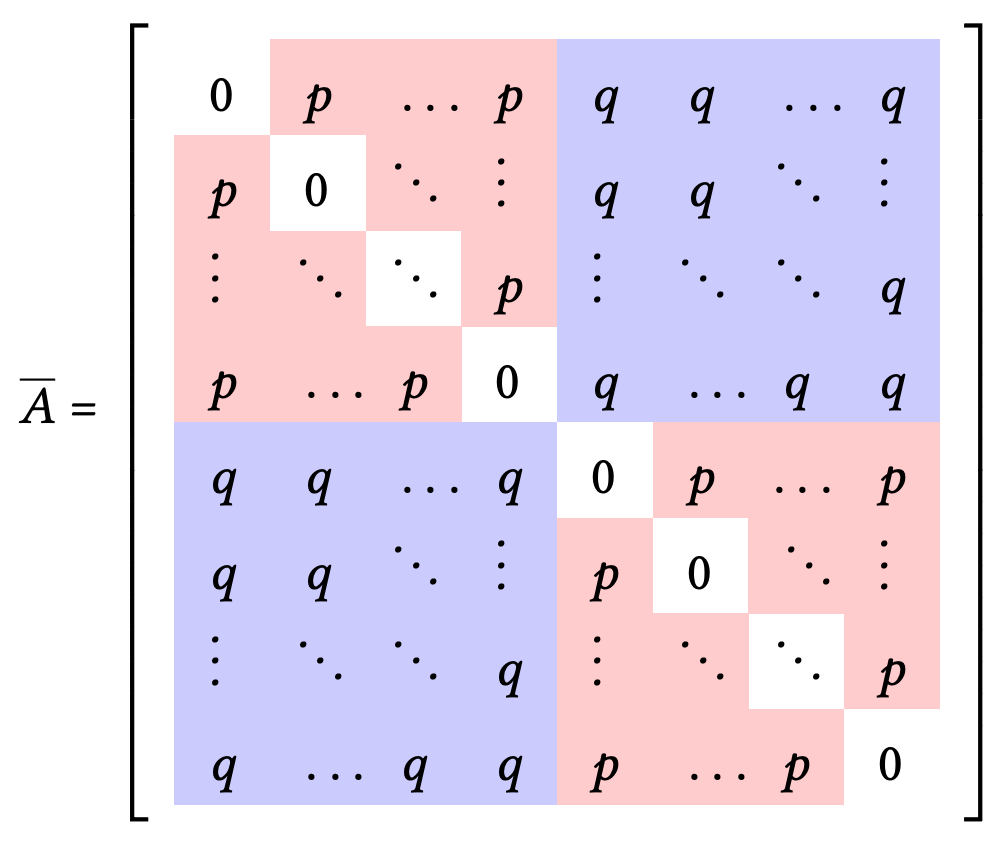
\includegraphics[scale=.2]{expectedA.png}
\end{figure}

Let $s$ be any mean-centered innate opinion vector
and let $z^*$ be the resulting equilibrium opinion
vector according to FJ dynamics.
Recall $z^* = (\bar{L}+I)^{-1}s$ where $\bar{L}$
is the Laplacian of $\bar{G}$.
Let $(\bar{L}+I)=\bar{U}\bar{S}\bar{U}$ where
$\bar{U}$ and $\bar{S}$ the eigendecomposition defined below.
Then
\begin{align}
    z^* = \frac{c_2}{2nq + 1} u^{(2)}
    + \frac{c_3}{nq +np + 1} u^{(3)}
    + \cdots + \frac{c_3}{nq +np + 1}u^{(3)} \nonumber
\end{align}
where $u^{(i)}$ is an eigenvector of $(\bar{L}+I)$ for
$i \in \{2, \ldots, 2n\}$.

\end{theorem}
\begin{proof}
Let $U' = \begin{bmatrix} u^{(1)} & u^{(2)} \end{bmatrix}$
where $u^{(1)}$
is the normalized all 1's vector and $u^{(2)}$
is the normalized vector with $n$ 1's followed
by $n$ -1's.
A back-of-the-envelope calculation shows that
$\bar{A} + p I=U'S'U'^T$
where $S' = \textrm{diag}(np+nq, np-nq)$.
Now, define $\bar{U} = \begin{bmatrix} u^{(1)} & u^{(2)} 
& Z \end{bmatrix}$,
where $Z \in \R^{2n \times (2n-2)}$ is a matrix
with orthonormal columns satisfying
$Z^T u^{(1)} = 0 = Z^T u^{(2)}$ built by
extending $u^{(1)}$ and $u^{(2)}$ to an orthonormal
basis.

With the observation that $\bar{U}\bar{U}^T
= \bar{U}^T \bar{U} = I$, we have:
\begin{align}\label{eq:decomposeLI}
    \bar{L}+I &= \bar{D} + I - \bar{A}
    = (np + nq)I + I - (\bar{A} + pI)
    \nonumber \\
    &= (np + nq + 1)I - U'S'U'^T
    = \bar{U}\bar{S}\bar{U}^T
\end{align}
where $\bar{S}=\textrm{diag}
(1, 2nq+1, np+nq+1, \ldots, np+nq+1)$.
Since $\bar{U}$ is an orthonormal basis, it follows that
$(\bar{L}+I)^{-1} = \bar{U}\bar{S}^{-1}\bar{U}$.
Additionally, because $\bar{U}$ is an orthonormal basis,
we can write: 
\begin{align}
    s = c_1 u^{(1)} + c_2 u^{(2)} 
    + \cdots + c_{2n} u^{(2n)}
    \nonumber
\end{align}
for scalars $c_i \in \R$
and columns $u^{(i)}$ of $\bar{U}$ 
where $i \in [2n]$.
Notice that $c_1 =0$ since $s$ is mean-centered.
Then we have that:
\begin{align}
    z^* = (\bar{L}+I)^{-1} s &= \bar{U}\bar{S}\bar{U}^T
    (c_2 u^{(2)} + c_3 u^{(3)} + \cdots + c_{2n} u^{(2n)})
    \nonumber \\
    &= \bar{U}\bar{S} \begin{bmatrix}
        0 & c_2 & c_3 & \cdots & c_{2n}
    \end{bmatrix}^T \nonumber \\
    &= \frac{c_2}{2nq + 1} u^{(2)}
    + \frac{c_3}{nq +np + 1} u^{(3)}
    + \cdots + \frac{c_3}{nq +np + 1}u^{(3)} \nonumber
\end{align}

\cref{thm:expectz} immediately follows.
\end{proof}

\subsection{Polarization Bounds}
We next present bounds for the polarization of the equilibrium
opinion resulting from FJ dynamics on any mean-centered
innate opinion vector. We extend the results of \cite{chitra20analyzing}
in the following ways:
\begin{itemize}
  \item Instead of requiring innate opinion vectors where the first block
  has opinion all 1 and the second block has opinion all -1,
  we allow for any mean-centered innate opinion vector.
  \item We consider the additional case of $q \geq p$. This case has real-world applications: for example, when dealing with opinion formation in a network of doctors and patients, opinions may be more likely to develop between doctors and patients
  than doctors and doctors or patients and patients.
  \item We explicitly describe the factors on the bound
  of polarization, and explain how they tighten as $n$ increases.
  \item We describe the special case $p=q$, equivalent to
  the Erdős-Rényi graph, and tightly characterize the bounds
  in this case.
\end{itemize}
Unfortunately, we trade the extension to any mean-centered
innate opinion to a limited result.
Instead of allowing $q \geq 1/n$, as in \cite{chitra20analyzing},
we require $q \geq p/2$.

\begin{theorem}\label{thm:converge}
  Let $G$ be a graph generated by the Stochastic Block Model
  with $p/2 \leq q \leq p$ and $p \geq C \log^4n/n$ or
  with $1/n \leq p \leq q$ and $q \geq C \log^4n/n$
  for some universal constant $C$.
  Let $s$ be any mean-centered innate opinion vector
  on $2n$ nodes and let $z^*$ be the equilibrium opinion
  vector according to FJ dynamics.
  Then for sufficiently large $n$,
  \begin{align}
    C' \frac{||s||_2^2}{(2nq+1)^2} \leq \Pz \leq
    C'' \frac{||s||_2^2}{(2nq+1)^2}
    \nonumber
  \end{align}
  with probability 97/100 where $C' \geq 1/6$
  and approaches $1/2$ as $n$ grows while
  $C'' \leq 16$ and approaches $4$ as $n$ grows.
\end{theorem}

\begin{proof}
At a high level, we prove \cref{thm:converge}
by writing $\Pz = s^T(L+I)^{-2}s$ 
and bounding the eigenvalues of $(L+I)^{-2}$
through clever comparisons to $\bar{L}$,
where $L$ is the Laplacian of $G$
and $\bar{L}$ is the Laplacian of the expected SBM $\bar{G}$.

First, notice that the normalized all 1's vector
$u^{(1)}$ is an eigenvector
of $(\bar{L}+I)$ by \cref{eq:decomposeLI}; $u^{(1)}$ is also an eigenvector
of $(L+I)$, since the columns and rows of $L$
must sum to 0 (by the definition of a graph Laplacian).
Unfortunately, $u^{(1)}$ has eigenvalue 1
for both $(L+I)^{-2}$ and $(\bar{L}+I)^{-2}$,
which poses a problem for the
bound we want to achieve.
We deal with this by
observing that $s$ is mean-centered and so
does not have any scaling of $u^{(1)}$.
It follows that
\begin{align}
    \Pz = s^T (L+I)^{-2} s = s^T (I-P)
    (L+I)^{-2}(I-P) s \nonumber
\end{align}
where $P$ is the projection $u^{(1)} {u^{(1)}}^T$.
The point of $(I-P)$ is to remove the eigenvector $u^{(1)}$
and corresponding eigenvalue 1.
Therefore, to bound $\Pz$, it is sufficient to
bound the eigenvalues of $(I-P)(L+I)(I-P)$, since
$s$ is some linear combination of the eigenvectors of
$(I-P)(L+I)(I-P)$.
To bound the eigenvalues of $(I-P)(L+I)(I-P)$,
we use \cref{lemma:boundL}, which tells us that the
eigenvalues of $L$ and $\bar{L}$ are within
$.5n\Mpq$ of each other for sufficiently large $n$.
We leave the proof of \cref{lemma:boundL} to
\cref{app:proof} for brevity.

\begin{lemma}[Extension of Lemma 4.5 in \cite{chitra20analyzing}]\label{lemma:boundL}
    Let $L$ be the Laplacian of graph $G$ drawn from
    the SBM and let $\bar{L} =\E[L]$. For fixed constant
    $C'$, with probability 98/100,
    \begin{align}
        ||L - \bar{L}||_2 \leq C' \sqrt{ n \log n \Mpq} \nonumber.
    \end{align}
\end{lemma}

Note that when $\Mpq \geq C \log^4 n /n$,
$C' \sqrt{ n \log n \Mpq} \leq \frac{C'}{\sqrt{C} \log^{1.5} n}
n \Mpq$.
So for $n \geq \exp(\frac{C'}{\sqrt{C}\epsilon})^{2/3}$,
$||L-\bar{L}||_2 \leq \epsilon n \Mpq$.
Choose $\epsilon = 1/2$.

From Weyl's Inequality and \cref{lemma:boundL}, we now have that
\begin{align}\label{eq:weyls}
    |\lambda_i - \bar{\lambda}_i| \leq ||L - \bar{L}||_2 \leq 
    \frac{1}{2} n \Mpq
\end{align}
for sufficiently large $n$,
where $\lambda_i$ is the $i$th eigenvalue of $L$ and 
$\bar{\lambda}_i$ is the $i$th eigenvalue of $\bar{L}$.
We now bound the largest $2n-1$ eigenvalues of $L+I$
or, equivalently, the eigenvalues of $(I-P)(L+I)(I-P)$.
The eigenvalues of $(I-P)(\bar{L}+I)(I-P)$ are $2nq+1$
and $np+nq+1$.

\paragraph{Case 1: \boldmath$q \geq p$}
The smallest eigenvalue of $(I-P)(\bar{L}+1)(I-P)$
is $nq+np+1 \geq nq+1$ while the largest eigenvalue is $2nq+1$.
Then, \cref{eq:weyls} implies that:
\begin{align}
    (.5nq + 1)(I-P)\preceq(I-P)(L+I)(I-P)\preceq(2.5nq+1)(I-P)
    \nonumber.
\end{align}
We square and invert each term, which yields:
\begin{align}
    (2.5nq + 1)^{-2}(I-P)\preceq(I-P)(L+I)^{-2}(I-P)
    \preceq(.5nq+1)^{-2}(I-P).
    \nonumber
\end{align}
Now, we can bound
\begin{align}
    \frac{1}{2} \frac{||s||_2^2}{(2nq+1)^2}
    \leq \frac{||s||_2^2}{(2.5nq+1)^2}
    \leq s^T(L+I)^{-2}s
    \leq \frac{||s||_2^2}{(.5nq+1)^2}
    \leq \frac{16||s||_2^2}{(2nq+1)^2}.
    \nonumber
\end{align}

\paragraph{Case 2: \boldmath$p \geq q \geq p/2$}
The smallest eigenvalue of 
$(I-P)(L+I)(I-P)$ is $2nq+1 \geq np+1$
while the largest eigenvalue is $nq+np+1 \leq 2np+1$.
Similar analysis to Case 1 yields
\begin{align}
    \frac{1}{6}\frac{||s||_2^2}{(2nq+1)^2}
    \leq \frac{||s||_2^2}{(2.5np+1)^2}
    \leq s^T(L+I)^{-2}s
    \leq \frac{||s||_2^2}{(.5np+1)^2}
    \leq \frac{16||s||_2^2}{(2nq+1)^2}.
    \nonumber
\end{align}
We now justify the
upper and lower bound on $C'$
and $C''$, respectively.
Consider a small $\epsilon$ such that
\cref{lemma:boundL} gives a small additive error.
Then, without loss of generality, the largest eigenvalue between Cases 1 and 2
is $(2+\epsilon)np+1$.
It follows that $C'$ gets arbitrarily close to $1/2$
as $n$ grows.
The smallest eigenvalue between Cases 1 and 2
$(1-\epsilon)np+1$ without loss of generality.
It follows that $C''$ gets arbitrarily close $4$
as $n$ grows.
\end{proof}

%\cref{thm:converge} applies to the SBM,
For $p=q$, the SBM
is simply an Erdős-Rényi random graph.
Therefore, a special case follows immediately
from \cref{thm:converge}.

\begin{theorem}[Erdős-Rényi Special Case]
    Let $G$ be a Erdős-Rényi graph where
    the probability of an edge between any pair
    of nodes is $p \geq C \log^4 n/n$ for some
    universal constant $C$.
    Let $s$ be any mean-centered innate opinion
    vector on $2n$ nodes
    and let $z^*$ be the equilibrium opinion vector
    according to $FJ$ dynamics.
    Then for sufficiently large $n$,
    \begin{align}
        C' \frac{||s||_2^2}{(2np+1)^2} \leq \Pz \leq
        C'' \frac{||s||_2^2}{(2np+1)^2}
        \nonumber
    \end{align}
    with probability 97/100 where $C' \geq 1/2$
    and $C'' \leq 2$. Both $C'$ and $C''$ approach
    1 as $n$ increases.
\end{theorem}

\begin{proof}
    The theorem immediately follows as a
    special case of \cref{thm:converge},
    except for the improved constants $C'$ and $C''$.
    To obtain the improved bounds, observe that
    the only eigenvalue of $(I-P)(L+I)(I-P)$
    is $2np+1$.
    Then, following the earlier analysis, we have that:
    \begin{align}
        \frac{1}{2}\frac{||s||_2^2}{(2np+1)^2}
        \leq \frac{||s||_2^2}{(2.5np+1)^2}
        \leq s^T(L+I)^{-2}s
        \leq \frac{||s||_2^2}{(1.5np+1)^2}
        \leq \frac{2||s||_2^2}{(2np+1)^2}.
        \nonumber
    \end{align}
    Setting $\epsilon$ to a small positive value
    yields an upper bound of $(2+\epsilon)np+1$
    on the eigenvalues and a lower bound
    of $(2-\epsilon)np+1$.
    It is easy to see that the factors
    $C'$ and $C''$ get arbitrarily close to 1
    as $\epsilon$ decreases.
    
\end{proof}

We remark that extending our results to the case of
$1/n \leq q \leq p/2$
would require bounding the inner product of the
largest $n-2$ eigenvectors, even if the innate opinion
vector $s$ did not have any scaling of the all 1's
vector or the second smallest eigenvector.



% chktex-file 46

\section{Conclusion}\label{sec:conclusion}
Filter bubbles are an important ethical issue.
Improving the mathematical theory behind their formation
presents an interesting and applicable area of research.
In this work, we empirically analyzed several
variations on the standard FJ dynamics opinion formation process
including the introduction of two natural
administrator actions.
Our theoretical contribution is a series of extensions
to the convergence bounds given by \cite{chitra20analyzing}.
Notably, we apply the bounds to any mean-centered
innate opinion vector and tightly characterize the
constraints when the Stochastic Block Model is in
the special case of the Erdős–Rényi graph.

\subsection{Future Work}

While answering some questions, our work points to several
avenues for future research:
The power of the theoretical bounds come from the natural
linear-algebraic description of FJ dynamics.
It would be interesting to write a network
administrator action in terms of a matrix multiplication.
Our main obstacle in this pursuit was balancing the
`macro' scale of any linear-algebraic action with
the `micro' scale employed in practice by social media platforms.
Bimodality is a natural and interesting alternative
measure of polarization.
However, the bimodality coefficient involves the third and fourth moments
of expectation.
While polarization can easily be represented as a quadratic measure,
cubic and quartic functions are more difficult to represent
in terms of vector operations.
An avenue for future research is either finding a
different measure or writing bimodality in a neat expression.

In terms of theory, we envision a way to give an explicit
expression for the bounds on the polarization convergence
in terms of the size of the network $n$.
We did not have sufficient time to write this up before
the deadline but hope to extend it later.

\subsection{Reflection and Responsibilities}
We enjoyed working on a problem at the intersection
of theoretical computer science and ethical issues.
It was satisfying to apply mathematical tools
to a problem facing the modern world.
Our greatest challenge was thinking of linear algebraic formulations of network administrator actions and bimodality; we ended up focusing on experimental results for these ideas, and have left them as interesting avenues for future work. 
However, we feel that we extended existing theoretical results
and introduced interesting variations to this problem, which we studied
empirically. 
It is our hope that we can publish this work or a future
iteration of it.
Finally, we thank Professor Chris Musco and Raphael Meyer for discussing this project with us and providing input on generating theoretical results. 


Responsibilities for the project and report:
Indu focused on related work, background, and processing
the data we used while
Teal coded the experiments and came up with the
theoretical extensions.
We collaborated on the abstract ideas of each section
and worked together to move through challenging parts
in the theoretical analysis.


\bibliography{references}
\bibliographystyle{plain}

\appendix
\section{Appendix}

\subsection{Proof of \cref{lemma:boundL}}\label{app:proof}

We introduce several lemmas that we will use to prove
\cref{lemma:boundL}.
Observe that this analysis closely follows that of
\cite{chitra20analyzing} except that we generalize it to
the case that $q\geq p$.

\begin{lemma}[Theorem 1.4 in \cite{vu05spectral}]\label{lemma:spectral}
    There are constants $C$ and $C'$ such that the following hold.
    Let $M_{i,j}$ be an independent random variable with mean
    0, variance at most $\sigma^2$ for $1 \leq i \leq j \leq m$,
    and absolute value bounded by $1$ where $\sigma \geq C' \sqrt{m} \log^2 m$.
    Then almost surely
    \begin{align}
        \lambda(M) \leq 2 \sigma \sqrt{m}
        + C \sqrt{\sigma} m^{1/4} \log m \nonumber
    \end{align}
    where $\lambda(M)$ denotes the spectral norm
    (i.e. maximum singular value) of $M$.
\end{lemma}

\begin{lemma}[Extension of Lemma 4.5 in \cite{chitra20analyzing}]\label{lemma:boundA}
    Let $A$ be the adjacency matrix of a graph drawn from the
    SBM with intra-block probability $p$ and inter-block
    probability $q$. Define $\bar{A} = \E[A]$.
    There exists a universal constant $C$ such that if
    $p \geq C \log^4 n/n$ then with probability 99/100,
    \begin{align}
        ||A - \bar{A}||_2 \leq 3\sqrt{n \Mpq} \nonumber.
    \end{align}
\end{lemma}

\begin{proof}[Proof (Omitted in \cite{chitra20analyzing})]
    Consider the matrix $M=A- \bar{A}$ with $m=2n$.
    Each entry $M_{i,j}$ for $i\neq j$ is a binary variable with
    probability $p$ or $q$ of firing.
    Recall that $M_{i,i}=0$.
    Then $\E[M_{i,j}] = \E[A_{i,j}] - \E[A]_{i,j} = 0$ and
    the variance $\sigma^2$ is less than $\Mpq$.
    The absolute value of each entry is bounded by 1,
    since every entry of $A$ is either 0 or 1,
    and every entry of $\bar{A}$ is between 0 and 1.
    We use that $1 \geq \sqrt{\Mpq} > \sigma$ and
    $\sqrt{\sigma} \geq C' (2n)^{1/4} \log 2n$.
    Then \cref{lemma:spectral} yields
    \begin{align}
        \lambda(A - \bar{A}) &\leq 2 \sqrt{\sigma} \sqrt{2n} +
        C \sqrt{\sigma} (2n)^{1/4} \log 2n \nonumber \\
        &\leq 2 \sqrt{\Mpq 2n} + \frac{C}{C'}\sqrt{\sigma}\sqrt{\sigma}
        \leq 3 \sqrt{n \Mpq} \nonumber
    \end{align}
    for sufficiently large $n$.
    Since $A - \bar{A}$ is a square matrix,
    $||A-\bar{A}|| \leq \lambda(A-\bar{A})$, which completes the proof.
\end{proof}

\begin{lemma}[Bernstein Inequality]\label{lemma:bernstein}
    Let $X_1, \ldots, X_m$ be independent random variables
    with variances $\sigma_1^2, \ldots, \sigma_m^2$ and
    $|X_i| \leq 1$ almost surely for $i \in [m]$.
    Let $X = \sum_{i \in [m]} X_i$, $\mu = \E[X]$,
    and $\sigma^2 = \sum_{i \in [m]} \sigma_i^2$.
    Then the following holds:
    \begin{align}
        \Pr (|X-\mu|>\epsilon) \leq \exp \left( \frac{e^2}
        {2\sigma^2 + \epsilon/3} \right) \nonumber
    \end{align}
\end{lemma}

With \cref{lemma:boundA} and \cref{lemma:bernstein},
we can now prove \cref{lemma:boundL}.


\begin{proof}[Proof of \cref{lemma:boundL}]
    Let $D$ be the degree matrix of $G$ and define
    $\E[D] = \bar{D}$. By the triangle inequality,
    $||L - \bar{L}||_2 \leq ||D - \bar{D}||_2 +
    ||A - \bar{A}||_2$.
    By \cref{lemma:boundA}, $||A - \bar{A}||_2 \leq
    3 \sqrt{n \Mpq}$.
    Additionally, $||D - \bar{D}||_2$ is bounded
    by $\max_{i \in [2n]} |D_{i,i} - \bar{D}_{i,i}|$.
    $D_{i,i}$ is a sum of Bernoulli random variables
    with total variance $\sigma^2$ upper bounded by
    $2 n \Mpq$. It follows from \cref{lemma:bernstein}
    and our assumption $p = \Omega(1/n)$ that
    $|D_{i,i} - \bar{D}_{i,i}| \leq C \sqrt{n \log n \Mpq}$
    with probability $1- 1/200n$ for
    fixed universal constant $C$.
    By a union bound, we have that
    $\max_i | D_{i,i} - \bar{D}_{i,i}| \leq \sqrt{n \log n \Mpq}$
    with probability 99/100.
    A second union bound with the event that
    $||A - \bar{A}||_2 \leq 3 \sqrt{n \Mpq}$ yields the lemma with
    $C' = C+1$.
\end{proof}

\section{Supplemental Material}

The code, data, and LaTeX files are all publicly
available at \href{https://github.com/rtealwitter/Filter-Bubbles}
{github.com/rtealwitter/Filter-Bubbles}.

The two data sets we use are described below:
\begin{itemize}
    \item Twitter is a graph with $548$ nodes and $3638$ edges. Nodes correspond to users who posted tweets about the Delhi legislative assembly elections of 2013, and edges represent user interactions debating that election. 
    \item Reddit is a graph with $556$ nodes and $8969$ edges. Nodes represent users who posted in the r/politics subreddit. Edges correspond to users' posts in different subreddits. In particular, two users are connected by an edge if they have both posted in two subreddits (other than r/politics) during the given time period.
\end{itemize}

\end{document}
